\documentclass[10pt]{article}
\usepackage[margin=0.8in]{geometry}
\usepackage{amsmath,amssymb}
\usepackage[T1]{fontenc}
\usepackage[utf8]{inputenc}
\usepackage{lmodern}
\usepackage{microtype}
\usepackage{enumitem}
\usepackage{booktabs}
\usepackage{array}
\usepackage{graphicx}
\usepackage{url}
\usepackage[hidelinks]{hyperref}
\def\UrlBreaks{\do\/\do\_\do-}
\setlist{nosep,leftmargin=1.3em}
\setlength{\parskip}{3pt}\setlength{\parindent}{0pt}
\sloppy
\newcommand{\fpath}[1]{\nolinkurl{#1}}
\newcolumntype{L}[1]{>{\raggedright\arraybackslash}p{#1}}
\setlength{\textfloatsep}{8pt plus 2pt minus 2pt}\setlength{\floatsep}{8pt plus 2pt minus 2pt}
\begin{document}

\begin{center}
{\Large\bfseries The MOND Acceleration Scale from MeerKAT: 47 Deep-Regime H\,{\sc i} Discs in MIGHTEE-HI COSMOS}\\[6pt]
{\small The authors --- draft for review, 2026-10-02, version 1.0 --- AI-assisted research programme; not peer reviewed}
\end{center}

% Conventions of this draft. Every number carried by an audit row of PAPER40_audit.py is checked against a committed file (git HEAD) or,
% for the rows marked "paper's own script", against PAPER40_figures_numbers.json written by make_paper40_figures.py (committed with this paper),
% and against the tex block that carries its tag. A line "% AUDIT: Bnn" after a paragraph, item, table or figure tags the audited numbers
% quoted in the text just above it (tags in text order). Numbers quoted only in running text are not checked by the script.
% The lanes are CFG301 (criteria 2555ab142, results 6b10c01c0), CFG302 (criteria 7d317dd4f, results a89ba33b9) and CFG304 (criteria 336b36f8f,
% results 34e40dac6). The post hoc rows of Section 5 are this paper's own diagnostics (make_paper40_figures.py), labelled as such wherever they appear.

\begin{abstract}
\noindent The programme ties the MOND acceleration scale to the vacuum, $a_0=\kappa c\sqrt{G\rho_\Lambda}$, with $\kappa=\tfrac12$ fitted, not derived; its footings are canonical $a_0=9.3603\times10^{-11}$ ($\rho_\Lambda$) and alternative $1.1312\times10^{-10}$\,m\,s$^{-2}$ ($\rho_{\rm crit}$). We run a framework-native width chain, frozen before any width was read, on the public MeerKAT MIGHTEE-HI COSMOS catalogue (293 H\,{\sc i} sources): $W_{50}$ and inclination give $V$, the baryons are $1.33\,M_{\rm HI}+M_\star$ at half the H\,{\sc i} diameter, and a median-residual estimator with the $\nu_{\rm mono}$ kernel returns $a_0$. 47 golden discs survive, all deep in the MOND regime ($g_{\rm bar}/a_0\le0.084$) and 37 gas-dominated; four calibration controls pass, among them a SPARC closure of the baryon side ($+0.008$\,dex). The pooled scale is $a_0=1.046\times10^{-10}$\,m\,s$^{-2}$ (bootstrap 68\% 1.01--1.15; recipe half-width $\pm0.143$\,dex): $+0.048$\,dex from the canonical footing, $-0.034$\,dex from the alternative and $-0.060$\,dex from SPARC's 1.20; $\kappa=0.56$ ($\rho_\Lambda$) or 0.46 ($\rho_{\rm crit}$). The direct $V^4/(GM_b)$ is $1.25\times10^{-10}$ (1.19 for the gas-dominated discs), which includes the kernel's next-order factor ($+0.078$\,dex). The dominant systematic is the H\,{\sc i} flux scale. The released cubes confirm the catalogue widths ($-0.022$\,dex, scatter 0.039\,dex) but hold less flux. Arecibo single-dish (ALFALFA) fluxes for 15 overlapping galaxies exceed the catalogue's by 0.195\,dex (the catalogue holds 0.64 of them) and the cubes' by more, so the cube scale is not supported; if that offset carried over to our fainter, more distant sample, $a_0$ would fall to about 0.6--0.75$\times10^{-10}$. On present evidence the flux scale places $a_0$ between about 0.6 and $1.05\times10^{-10}$, the catalogue value at the top; the velocity frame of the catalogue widths could add $+0.098$\,dex. On the catalogue's flux scale the result is consistent with SPARC and with both footings, on the single-dish scale below both. It does not separate the footings and, at $z\le0.093$, cannot test the constant $a_0(z)$ the framework predicts (the rival's lever is 0.009\,dex). The cold mass ($\Omega_ch^2\approx0.12$) is still required.
\end{abstract}
% AUDIT: B01

\section{Introduction}\label{sec:intro}

\textbf{The relation and its scale.} Milgrom's modified dynamics [M83] replaces the Newtonian acceleration below a scale $a_0$. In rotating galaxies the observed centripetal acceleration $g_{\rm obs}$ follows the baryonic one $g_{\rm bar}$ along a single radial acceleration relation: 2693 points in 153 SPARC galaxies [LMS16, MLS16, L17], with SPARC's fitted scale $g_\dagger=1.20\times10^{-10}$\,m\,s$^{-2}$ [MLS16]. A full joint inference over the SPARC distances, inclinations, luminosities and mass-to-light ratios finds $a_0=(1.19\pm0.04\,{\rm(stat)}\pm0.09\,{\rm(sys)})\times10^{-10}$\,m\,s$^{-2}$ [D23].
% AUDIT: B02

\textbf{MeerKAT.} The MIGHTEE-HI survey [MM26] measures H\,{\sc i} out to $z\approx0.09$ with one instrument and one pipeline. From its early-science data, Ponomareva et al.\ [P21] built the H\,{\sc i} baryonic Tully--Fisher relation of 67 galaxies from both the global-profile width $W_{50}$ and resolved rotation curves, and found no evolution over $0\le z\le0.081$. Rajohnson et al.\ [R22] measured the H\,{\sc i} size--mass relation of 204 galaxies (slope 0.501, intercept $-3.252$). V\u{a}r\u{a}\c{s}teanu et al.\ measured the radial acceleration relation with resolved, SED-based stellar mass-to-light ratios, first in 19 H\,{\sc i}-selected galaxies to $z=0.08$ [V25], then in 130 resolved MIGHTEE-HI and LADUMA galaxies to $z\approx0.09$ [V26], finding $a_0=(1.50\pm0.05)\times10^{-10}$\,m\,s$^{-2}$ with their kernel and mass modelling and no significant redshift evolution. The MIGHTEE-HI COSMOS catalogue [MM26] lists 293 sources at $0.004<z<0.093$ with H\,{\sc i} masses, $W_{50}$ widths, inclinations and stellar masses.
% AUDIT: B03

\textbf{The framework.} The programme ties the scale to the vacuum energy density, $a_0=\kappa c\sqrt{G\rho_\Lambda}$, with $\kappa=\tfrac12$ fitted, not derived. With $H_0=67.4$\,km\,s$^{-1}$\,Mpc$^{-1}$ and $\Omega_\Lambda=0.6847$ [PL20] this gives the canonical footing $a_0=9.3603\times10^{-11}$\,m\,s$^{-2}$; the same coefficient on the critical density gives the alternative footing $1.1312\times10^{-10}$. Its galaxy law is a MOND kernel $\nu$ with $g_{\rm obs}=\nu(g_{\rm bar}/a_0)\,g_{\rm bar}$. The framework's own closed form, $\nu=\sqrt{1+a_0/g_{\rm bar}}$, is the relation contained in Milgrom's vacuum-effect paper [M99] (with a different coefficient); the measurement lanes use the monotone kernel $\nu_{\rm mono}$, which below $g_{\rm bar}/a_0=2.54$ equals the exponential form $\nu=[1-\exp(-\sqrt{y})]^{-1}$ ($y=g_{\rm bar}/a_0$) to $2\times10^{-4}$. That form is the $\alpha=\tfrac12$ member of the family of Milgrom \& Sanders [MS08] and the fitting function of [MLS16]. The distinctive prediction is a constant $a_0(z)$; the rival reading $a_0\propto H(z)$ rises by a factor $E(z)$. The framework adds no dark-matter particle, but the cold mass ($\Omega_ch^2\approx0.12$) is still required for cosmology.
% AUDIT: B04

\textbf{This paper.} We report a framework-native, catalogue-based measurement of the local $a_0$ from MIGHTEE-HI (lane CFG301), with criteria frozen and committed before any width, velocity or mass value was read, four calibration controls that could fail, a re-measurement of the inputs from the released cubes (lane CFG302) and an independent check of the H\,{\sc i} flux scale against Arecibo single-dish fluxes (lane CFG304). No halo model enters; the only cosmological input is the catalogue's luminosity distance.

\section{Data}\label{sec:data}

\textbf{The catalogue.} The MIGHTEE-HI COSMOS catalogue [MM26] gives, per source: $z_{\rm HI}$; the luminosity distance $D_L$ (flat $\Lambda$CDM, $H_0=70$, $\Omega_M=0.3$, no peculiar-velocity correction); $\log M_{\rm HI}$; the 3-D signal-to-noise $S\!N_{\rm 3D}$; $W_{50}$ from a busy-function fit [W14] at 50\% of the peak, not corrected for inclination; the inclination from $g$-band isophotes with intrinsic thickness $q_0=0.2$; the stellar mass from BAGPIPES SED fits [C18]; and five quality flags (low confidence, blended, confused, bad ellipse, contaminated). The \emph{golden sample} has all five flags zero. The catalogue's distances agree with flat $\Lambda$CDM at $H_0=70$ to 0.45\% over the survivors, and its inclinations follow from its axis ratios with $q_0=0.2$ to 0.8$^\circ$ (rounding; this paper's script).
% AUDIT: B05

\textbf{The frozen cut.} Applied by code, in this order, before any width was read as data: the golden sample (293 to 202 sources); $0.02\le z_{\rm HI}\le0.093$ (188; a 300\,km\,s$^{-1}$ peculiar velocity is then at most 5\% of the distance); $45^\circ\le i\le80^\circ$ (122); $\log M_{\rm HI}\ge9.0$ (78); $W_{50}\ge80$\,km\,s$^{-1}$ with $\sigma_{W_{50}}/W_{50}\le0.15$ (70); $S\!N_{\rm 3D}\ge8$ (47); finite inputs (47). The 47 survivors are split by redshift into three equal-count windows: W1 (16 galaxies, $z$ 0.0266--0.0476, median 0.042, median $D_L$ 185\,Mpc), W2 (16, $z$ 0.0506--0.0756, median 0.067, 300\,Mpc) and W3 (15, $z$ 0.0773--0.0930, median 0.081, 368\,Mpc). The median gas fraction is 0.70.
% AUDIT: B06

\section{Method}\label{sec:method}

\textbf{The chain.} For each galaxy,
\begin{equation*}
V=\frac{W_{50}-\delta}{2(1+z)\sin i},\qquad M_b=1.33\,M_{\rm HI}+M_\star,\qquad R=\tfrac12D_{\rm HI},\quad \log_{10}\frac{D_{\rm HI}}{\rm kpc}=0.506\log_{10}\frac{M_{\rm HI}}{\rm M_\odot}-3.293,
\end{equation*}
\begin{equation*}
g_{\rm bar}=\frac{GM_b}{R^2},\qquad g_{\rm obs}=\frac{V^2}{R},\qquad D=\frac{g_{\rm obs}}{g_{\rm bar}},
\end{equation*}
with $\delta=0$ (the primary; a turbulence term $\delta=11$\,km\,s$^{-1}$ is a recipe knob), the catalogue inclination, the factor 1.33 for helium, no molecular gas, and the BAGPIPES $M_\star$. The size relation has the form of Wang et al.\ [W16]; its coefficients are those adopted in the programme's earlier width lane (CFG260) and were not re-checked against [W16] here. All baryons are placed inside $R$ as a point mass.
% AUDIT: B07

\textbf{The estimator.} The implied ratio $s^*$ is the root of $\mathrm{median}_i\,\log_{10}[D_i/\nu(g_{{\rm bar},i}/(a_0s))]=0$ with $\nu=\nu_{\rm mono}$ and $a_0$ the canonical value; the measured scale is $s^*\times9.3603\times10^{-11}$\,m\,s$^{-2}$ (the alternative footing gives the same absolute $a_0$ to $7\times10^{-17}$\,dex). Intervals come from a bootstrap over galaxies ($B=4{,}000$). In the deep limit $\nu\to y^{-1/2}$ and the estimator reduces to $a_0=V^4/(GM_b)$, independent of $R$; at the next order a galaxy on the law shows $V^4/(GM_b)=a_0\,y\,\nu(y)^2>a_0$, and the estimator removes that factor.
% AUDIT: B08

\textbf{The recipe half-width} is the quadrature of four knobs, each applied to every galaxy: $\delta=11$\,km\,s$^{-1}$; $M_\star\pm0.25$\,dex; $D_{\rm HI}$ (hence $R$) $\pm0.15$\,dex; and the distances moved from $H_0=70$ to 67.4 (the value behind $\rho_\Lambda$). The isotropic $\sin60^\circ$ in place of the catalogue inclinations is reported as a sensitivity. A second statistic, frozen with the first, is the direct ratio $a_0^{\rm BTFR}=V^4/(GM_b)$ per galaxy, with its median over (i) all survivors, (ii) the gas-dominated discs ($1.33\,M_{\rm HI}>M_\star$) and (iii) the deep discs ($y<0.5$).
% AUDIT: B09

\textbf{Calibration controls (frozen; evaluated before any $a_0$ was printed; each could fail).}
\begin{itemize}
\item \emph{CC1, local level:} the nearest window W1 must return $s^*$ within $\pm0.15$\,dex of the SPARC scale ($1.20/0.93603=1.282$) and of the programme's ALFALFA control (CFG281, $s^*=1.449$ [H18, D20]), with a recipe half-width $\le0.20$\,dex. W1 gives $s^*=1.233$: $-0.017$\,dex from 1.282, $-0.070$\,dex from 1.449, half-width 0.136. PASS.
\item \emph{CC2, SPARC closure of the baryon side:} the same $M_b$ (with $0.5\,L_{[3.6]}$ for the stars), size relation and point mass applied to 123 SPARC galaxies (quality $\le2$, $i\ge30^\circ$, $V_{\rm flat}>0$) with $g_{\rm obs}=V_{\rm flat}^2/R$ return $s^*=1.304$, $+0.008$\,dex from 1.282. With the measured $R_{\rm HI}$ in place of the relation the value is 1.324; the relation is unbiased on SPARC (median $-0.002$\,dex). PASS.
\item \emph{CC3, drift:} $|\log s^*({\rm W3})-\log s^*({\rm W1})|\le0.10$\,dex. The drift is $-0.057$\,dex. PASS, with little power: the statistical width of the drift is 0.136\,dex.
\item \emph{CC4, self-test:} in 100 worlds with widths fabricated from the law at $s=2$ on the survivors' own masses and inclinations (0.15\,dex scatter, 10\% width errors), the bias is $-0.013$\,dex (tolerance 0.023) and the 95\% interval covers the truth in 93 of 100. PASS.
\end{itemize}
% AUDIT: B10

\textbf{Reactivity and reproduction.} Widths multiplied by 1.1892 raise the pooled $s^*$ by $+0.322$\,dex (expected $0.30\pm0.05$; MUTATE=1); $\sin i_{\rm eff}=0.70$ against the $\sin60^\circ$ variant raises it by $+0.392$\,dex (expected $0.37\pm0.06$; MUTATE=2). The chain, fed CFG281's ALFALFA arrays, reproduces CFG281's committed $s^*$ exactly (1.332408 unmatched, 1.449173 matched; M5). All six frozen hand estimates hit. An independent re-run reproduced every results file identically.
% AUDIT: B11

\textbf{Disclosures.} Before the freeze only the catalogue's header line had been read. The frozen text asks for mass-matched windows in CC1 and CC3 but does not define the matching; the rule fixed in the script before any value was read (W1 and W2 matched to W3's $\log M_{\rm HI}$ quartile bins, at least three galaxies per bin) could not be met (W1 had 8/3/2/2 galaxies per bin), so CC1, CC3 and the drift use unmatched windows. W1's median $\log M_{\rm HI}$ (9.605) is 0.155\,dex below W3's (9.76). A reader who insists on matching should treat CC1 and CC3 as not evaluable; the calibrated label then rests on CC2 and the unmatched numbers. The BTFR kernel-factor diagnostic was added after the SPARC control and before the measurement, using baryons only.
% AUDIT: B12

\section{Results}\label{sec:results}

\begin{table}[t]
\centering\small
\setlength{\tabcolsep}{4pt}
\begin{tabular}{lcccccccc}
\toprule
set & $N$ & $z$ median & $D_L$ [Mpc] & $s^*$ & $a_0$ [$10^{-10}$ m s$^{-2}$] & 68\% & 95\% & recipe [dex] \\
\midrule
W1 & 16 & 0.042 & 185 & 1.233 & 1.154 & 1.045--1.312 & 0.964--1.910 & 0.136 \\
W2 & 16 & 0.067 & 300 & 1.089 & 1.019 & 0.931--1.153 & 0.768--1.311 & 0.139 \\
W3 & 15 & 0.081 & 368 & 1.081 & 1.012 & 0.780--1.336 & 0.467--1.424 & 0.135 \\
pooled & 47 & --- & --- & 1.117 & 1.046 & 1.012--1.145 & 0.936--1.311 & 0.143 \\
\bottomrule
\end{tabular}
\caption{The implied $a_0$ per redshift window and pooled (CFG301; $s^*=a_0/9.3603\times10^{-11}$). The 68\% and 95\% columns are bootstrap intervals over galaxies, in $10^{-10}$\,m\,s$^{-2}$; the recipe column is the half-width of the four-knob quadrature.}
\label{tab:res}
\end{table}
% AUDIT: B13

\textbf{The level.} The pooled scale is $a_0=1.046\times10^{-10}$\,m\,s$^{-2}$ ($s^*=1.117$), with a bootstrap 68\% interval of 1.012--1.145 and a 95\% interval of 0.936--1.311, and a recipe half-width of 0.143\,dex (Table~\ref{tab:res}, Fig.~\ref{fig:levels}). It lies $+0.048$\,dex above the canonical footing, $-0.034$\,dex below the alternative and $-0.060$\,dex below SPARC's 1.20. The recipe knobs contribute 0.106 ($\delta$), 0.086 ($M_\star$), 0.026 ($D_{\rm HI}$) and 0.036\,dex ($H_0$); the $\sin60^\circ$ sensitivity is 0.026\,dex (0.146 with it in the quadrature). All 47 galaxies are deep: $y=g_{\rm bar}/a_0$ at $R$ has quartiles 0.028, 0.033 and 0.042 and a maximum of 0.084.
% AUDIT: B14

\textbf{The windows and the drift.} The window medians are 1.154, 1.019 and 1.012 (Table~\ref{tab:res}); their bootstrap intervals are lumpy, because a median of 15--16 galaxies jumps between galaxies. The slope of $\log_{10}s^*$ on $\log_{10}D_L$ is $-0.20$ per dex (68\% $-0.67$ to $+0.08$; 95\% $-1.25$ to $+0.35$): not resolved. The ratio W3/W1 is 0.877 ($\log_{10}$: $-0.057\pm0.136$). The programme's ALFALFA control falls by 0.105\,dex between 20--50 and 50--85\,Mpc (CFG281), the same sign. Between W1 and W3 the rival $a_0\propto H(z)$ predicts $+0.009$\,dex, far below the statistical width.
% AUDIT: B15

\textbf{The direct BTFR.} The median $V^4/(GM_b)$ is $1.251\times10^{-10}$\,m\,s$^{-2}$ over all 47 (68\% 1.187--1.348; $+0.126$\,dex from the canonical footing, $+0.044$\,dex from the alternative; recipe 0.123\,dex) and $1.187\times10^{-10}$ over the 37 gas-dominated discs (68\% 1.109--1.251; $+0.103$ and $+0.021$\,dex; recipe 0.128\,dex). The deep subset (iii) is the same 47 galaxies as (i). These rows sit above the $s^*$ row by design: computed from the baryons alone, the median kernel factor $y\nu_{\rm mono}(y)^2$ is 1.197 ($+0.078$\,dex) at the canonical $a_0$ and 1.172 at $1.20\times10^{-10}$, and 1.183 for the gas-dominated discs. The gas-dominated median differs from the full one by $-0.023$\,dex, so the stellar mass hardly matters. The same recipe on SPARC gives a BTFR level of $1.526\times10^{-10}$ (CC2's diagnostic). Fig.~\ref{fig:btfr} shows the 47 discs against the deep-MOND line on both footings.
% AUDIT: B16

\textbf{The coefficient.} Read as $\kappa=\tfrac12\,a_0/a_0^{\rm footing}$, the pooled scale gives $\kappa=0.559$ on the $\rho_\Lambda$ footing (bootstrap 68\% 0.540--0.612, 95\% 0.500--0.701; scaled by $10^{\pm0.143}$, 0.40--0.78) and $\kappa=0.462$ on $\rho_{\rm crit}$ (68\% 0.447--0.506, 95\% 0.414--0.580; recipe 0.33--0.64). On statistics alone $\kappa=\tfrac12$ sits at the lower edge of the 95\% interval on the $\rho_\Lambda$ footing and inside the 68\% interval on $\rho_{\rm crit}$; with the recipe width it is inside both. These are on the catalogue's $H_0=70$ distances. On the $H_0=67.4$ distances that match $\rho_\Lambda$, the scale falls by 0.036\,dex and the central values become 0.514 and 0.425 (Section~\ref{sec:sys}).
% AUDIT: B17

\textbf{Against other determinations.} The pooled scale is $-0.056$\,dex from the joint inference of [D23] (1.19) and $-0.157$\,dex from the MIGHTEE-HI/LADUMA resolved fit of [V26] (1.50), which uses resolved rotation curves, resolved SED mass-to-light ratios and its own kernel; the authors' sub-samples span 1.31--1.80 (CFG279). The two MIGHTEE values are not the same measurement: ours places all baryons at $D_{\rm HI}/2$ and reads the velocity from $W_{50}$, and the samples overlap only in part (not checked galaxy by galaxy). Which H\,{\sc i} flux scale the resolved analysis uses we have not checked.
% AUDIT: B18

\begin{figure}[t]
\centering
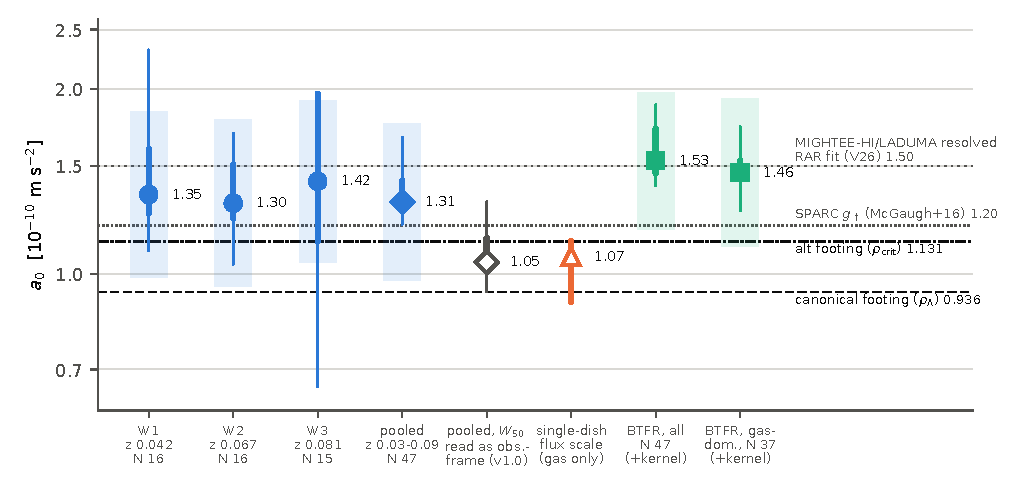
\includegraphics[width=\linewidth]{fig1_paper40_levels.pdf}
\caption{The implied $a_0$ of CFG301 per redshift window (circles) and pooled (filled diamond), with bootstrap 68\% (thick) and 95\% (thin) intervals and the recipe half-width (shaded box). Open markers: the pooled value on the Arecibo single-dish flux scale (CFG304's interpolation of CFG301's band rows, with the 68\% range of its flux ratio), all baryons raised (A, 0.60; 0.50--0.68) or the gas alone (B, 0.70; 0.61--0.76). Squares: the direct BTFR medians, which include the kernel's next-order factor ($+0.078$\,dex). Lines: the canonical (0.936) and alternative (1.131) footings, SPARC's fitted $g_\dagger$ (1.20) and the MIGHTEE-HI/LADUMA resolved fit with the authors' mass modelling (1.50), in $10^{-10}$\,m\,s$^{-2}$.}
\label{fig:levels}
\end{figure}
% AUDIT: B19

\begin{figure}[t]
\begin{minipage}[c]{0.54\linewidth}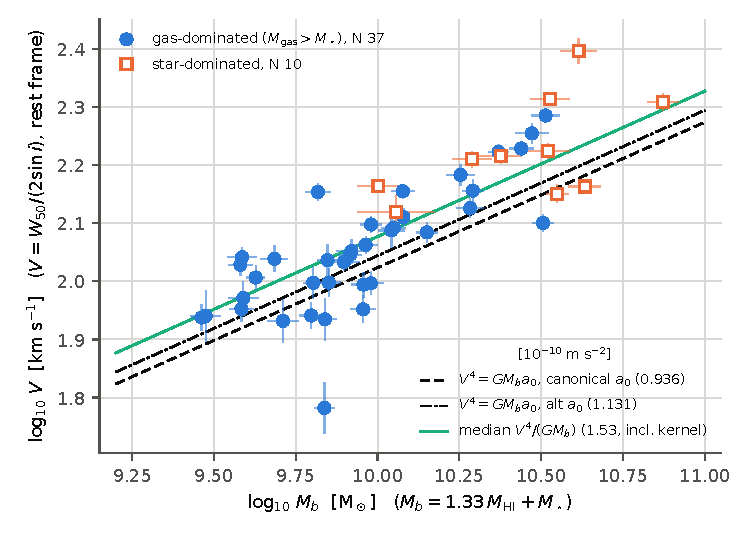
\includegraphics[width=\linewidth]{fig2_paper40_btfr.pdf}\end{minipage}\hfill
\begin{minipage}[c]{0.43\linewidth}\small
\caption{The 47 discs in the plane of $V=W_{50}/[2(1+z)\sin i]$ and $M_b=1.33\,M_{\rm HI}+M_\star$: gas-dominated (filled, 37) and star-dominated (open, 10). Error bars: the catalogue's $W_{50}$ error and the quadrature of its $M_{\rm HI}$ and $M_\star$ errors; inclination errors are not tabulated and not shown. Lines: $V^4=GM_ba_0$ on the canonical and alternative footings (the deep-MOND limit) and the median $V^4/(GM_b)=1.25\times10^{-10}$\,m\,s$^{-2}$, which includes the kernel factor.}
\label{fig:btfr}\end{minipage}
\end{figure}
% AUDIT: B20

\section{Systematics}\label{sec:sys}

\begin{table}[t]
\centering\footnotesize
\setlength{\tabcolsep}{4pt}
\begin{tabular}{L{0.56\linewidth}cL{0.22\linewidth}}
\toprule
variant (all on the same 47 discs) & $\Delta\log_{10}a_0$ [dex] & source \\
\midrule
H\,{\sc i} flux scale at the single-dish level (catalogue/ALFALFA $-0.195$\,dex): all baryons raised, band interpolation & $-0.243$ & CFG304 \\
same, gas alone (gas fraction 0.70), band interpolation & $-0.174$ & CFG304 \\
same, all baryons raised at fixed $R$, exact re-run & $-0.237$ & post hoc, this paper \\
same, gas alone, $R$ from the size relation, exact re-run & $-0.144$ & post hoc, this paper \\
same, the 7 matched pairs that pass CFG301's cut ($-0.159$\,dex): all baryons / gas alone & $-0.193$ / $-0.141$ & CFG304 post hoc \\
velocity frame: catalogue $W_{50}$ read as rest-frame (no $1+z$) & $+0.098$ & post hoc, this paper \\
inclination: $q_0=0.10$ / $0.30$ in place of 0.2 & $+0.025$ / $-0.055$ & post hoc, this paper \\
inclination: isotropic $\sin60^\circ$ & $+0.026$ & CFG301 \\
turbulence $\delta=11$\,km\,s$^{-1}$ & $-0.106$ & CFG301 recipe \\
stellar mass $\pm0.25$\,dex & $-0.090$ / $+0.082$ & CFG301 recipe \\
$D_{\rm HI}$ $\pm0.15$\,dex & $+0.021$ / $-0.031$ & CFG301 recipe \\
MIGHTEE's own size relation [R22] & $-0.001$ & post hoc, this paper \\
distances on $H_0=67.4$ instead of 70 & $-0.036$ & CFG301 recipe \\
\bottomrule
\end{tabular}
\caption{Systematic variants of the pooled $a_0$ ($1.046\times10^{-10}$). Post hoc rows are this paper's script (\fpath{make_paper40_figures.py}), which first reproduces CFG301's committed pooled, window, band, $H_0$ and BTFR values exactly; they were not frozen. The single-dish rows are a signed systematic for galaxies brighter and nearer than ours, not a measurement.}
\label{tab:sys}
\end{table}
% AUDIT: B21

\textbf{The H\,{\sc i} flux scale (CFG302).} CFG302 re-measured the 188 golden sources at $0.02\le z\le0.093$ from the four released MIGHTEE-HI r1p0 cubes (circular restoring beam 74.2--77.3$''$, 8$''$ pixels), with criteria frozen before any spectrum was extracted. Of the 179 sources in its primary set, 58 reach its frozen detection threshold. \emph{The widths agree:} the median log ratio of our rest-frame $W_{50}$ to the catalogue's is $-0.022$\,dex with a robust scatter of 0.039\,dex (4 of 58 pull outliers), so the velocity side of the chain stands. \emph{The fluxes do not:} the median ratio over all 179 is 0.22, and over the 58 detections the median log ratio is $-0.30$\,dex (a ratio of 0.50, scatter 0.24\,dex; 46 of 58 pull outliers). The aperture is complete ($S(2.5\theta)/S(1.5\theta)=1.002$), and the stacked line holds $0.60\pm0.05$ of the catalogue's mean flux. One frozen control failed and is kept: the line-free signal-to-noise spread is 0.489, not about 1, because the noise is anticorrelated over long spectral lags, as if the released spectra were high-pass filtered. For exactly our 47 discs (post hoc join with CFG302's committed table), 45 are in its primary set and 20 reach its threshold; their median cube-to-catalogue flux log ratio is $-0.443$\,dex, while their widths agree ($-0.017$\,dex).
% AUDIT: B22

\textbf{An independent flux scale (ALFALFA, CFG304).} CFG304 matched the catalogue with the ALFALFA catalogue of Arecibo single-dish fluxes [H18], under criteria frozen before any per-galaxy flux was read: 23 matches, 15 of them ALFALFA code 1. The matches are real: catalogue and ALFALFA widths agree to $+0.000$\,dex (scatter 0.037), and shuffled positions give 0.275 matches on average. On the 15 code-1 pairs the median log ratio of catalogue to single-dish flux is $-0.195$\,dex (68\% $-0.250$ to $-0.156$), a ratio of about 0.64; for the 7 of them with a cube detection the cube ratio is $-0.308$\,dex. Without pairs that have a catalogued neighbour within 3.5$'$ the two ratios are $-0.175$ and $-0.383$. The catalogue's $\log M_{\rm HI}$ sit 0.22\,dex below ALFALFA's for the same galaxies, consistent with the flux ratio. The frozen decision is ``neither'': the single dish sees more H\,{\sc i} than both MeerKAT scales, and the cube scale lies further from it than the catalogue's, so the cube scale is not the relevant systematic. The deficit persists at $z\ge0.02$ ($-0.137$\,dex over 19 pairs, post hoc). Its cause is open: losses in the catalogue's 3$\sigma$ masks, the released products, the absolute flux scale, or Arecibo's 3.5$'$ beam adding flux from uncatalogued neighbours.
% AUDIT: B23

\textbf{What the flux scale does to $a_0$.} The chain uses the catalogue's $M_{\rm HI}$. If the single-dish scale applied to our 47 discs, their H\,{\sc i} masses would rise by about 0.2\,dex and $a_0$ would fall. CFG304's interpolation of CFG301's band rows gives $5.97\times10^{-11}$ with all baryons raised (68\% 4.98--6.76) and $7.00\times10^{-11}$ with the gas alone at a gas fraction of 0.70 (68\% 6.08--7.60). Exact re-runs of the chain (post hoc) give $6.06\times10^{-11}$ (all baryons, fixed $R$) and $7.50\times10^{-11}$ (the gas alone, each galaxy's own gas fraction, $R$ following the size relation; 7.11 at fixed $R$). The 7 matched pairs that pass CFG301's own cut have a ratio of $-0.159$\,dex, which gives 6.7 and $7.6\times10^{-11}$ (CFG304, post hoc). This is a signed systematic, not a measurement: the matched galaxies are the 23 H\,{\sc i}-brightest COSMOS sources at $z\le0.047$, while our 47 reach $z=0.093$, mostly beyond ALFALFA, so whether the offset carries over is an assumption. On present evidence the flux scale places $a_0$ between about 0.6 and $1.05\times10^{-10}$, with the catalogue-scale value at the top. On the single-dish scale $\kappa$ would be 0.32--0.40 ($\rho_\Lambda$) or 0.26--0.33 ($\rho_{\rm crit}$), below $\tfrac12$ on both footings, and $a_0$ would sit 0.20--0.30\,dex below SPARC's 1.20.
% AUDIT: B24

\textbf{The velocity frame.} The chain divides $W_{50}$ by $1+z$, reading the catalogue widths as observed-frame. CFG302's raw widths agree with that reading to $+0.002$\,dex and with the rest-frame reading to $-0.022$\,dex, which does not decide the convention ($\pm0.025$\,dex). If the catalogue widths were already rest-frame, the pooled $a_0$ would rise by 0.098\,dex to $1.31\times10^{-10}$ (post hoc; median $z=0.065$).
% AUDIT: B25

\textbf{Inclinations, turbulence, stellar mass and size.} The catalogue's inclinations follow from its axis ratios with $q_0=0.2$; $q_0=0.10$ or 0.30 moves the pooled $a_0$ by $+0.025$ or $-0.055$\,dex (post hoc) and the isotropic $\sin60^\circ$ by $+0.026$\,dex, and the $45^\circ$ cut keeps the face-on end, where $\sin i$ errors are largest, out. No turbulence correction is applied; $\delta=11$\,km\,s$^{-1}$, the largest recipe term, lowers $a_0$ by 0.106\,dex. The stellar mass enters weakly because 37 of the 47 discs are gas-dominated ($\pm0.25$\,dex on $M_\star$: $-0.090$ / $+0.082$\,dex). In the deep limit the estimator does not depend on $R$, so the size relation enters only at next order: $D_{\rm HI}\pm0.15$\,dex moves $a_0$ by 0.026\,dex (half-width), and MIGHTEE's own relation [R22] by $-0.001$\,dex ($D_{\rm HI}$ smaller by 0.008\,dex at the median $\log M_{\rm HI}=9.73$). The point mass at $D_{\rm HI}/2$ is a recipe choice that CC2 tests on SPARC, not a resolved mass model.
% AUDIT: B26

\textbf{Distances and $H_0$.} The catalogue's distances assume $H_0=70$ and no peculiar velocities, while $\rho_\Lambda$ uses $H_0=67.4$. Moving the distances to 67.4 raises every mass by $2\log_{10}(70/67.4)$ and lowers the pooled $a_0$ by 0.036\,dex, to $9.62\times10^{-11}$ ($s^*=1.028$). This is a convention, not an error; quoted alone, the result is on the catalogue's distances. Peculiar velocities are random per galaxy and at most 5\% in distance above $z=0.02$.
% AUDIT: B27

\textbf{Mass matching and sample size.} The windows could not be mass-matched (Section~\ref{sec:method}), so the drift compares W1, whose median $\log M_{\rm HI}$ is 0.155\,dex lower, with W3. With 15--16 galaxies per window the window medians are lumpy (W3's 95\% interval spans a factor of three), CC3 has little power and the drift slope is unresolved. The sample is H\,{\sc i}-selected and mass-limited at high $z$.
% AUDIT: B28

\section{What the result can and cannot say}\label{sec:say}

\begin{itemize}
\item \textbf{It can say:} an independent instrument and sample, with no halo model and a chain calibrated on SPARC, give a deep-regime scale of $1.046\times10^{-10}$\,m\,s$^{-2}$ on the catalogue's flux scale, the top of the flux-scale range. That is consistent with SPARC ($-0.060$\,dex) and with both of the framework's footings, and $\kappa=\tfrac12$ lies inside the recipe width on both.
\item \textbf{It is not a footing discriminator.} The footings differ by 0.082\,dex; the result sits between them, $+0.048$ and $-0.034$\,dex away, with a recipe half-width of 0.143\,dex and a single-dish flux systematic of $-0.14$ to $-0.24$\,dex.
\item \textbf{It is not an $a_0(z)$ test.} At $z\le0.093$ the rival $a_0\propto H(z)$ differs from a constant by 0.009\,dex between W1 and W3, against a statistical width of 0.136\,dex. The distinctive constant-$a_0(z)$ prediction needs $z\gtrsim2$ and baryon calibrations near 0.1\,dex [P38].
\item \textbf{It is conditional on the flux scale.} If the single-dish offset applies to our discs, the same chain gives 0.60--0.75$\times10^{-10}$, below both footings and 0.20--0.30\,dex below SPARC, an offset that the chain's SPARC closure (CC2, $+0.008$\,dex) does not show. Whether it applies to galaxies fainter and more distant than the matched ones is open; it needs single-dish or total-power fluxes for the CFG301 sample itself.
\item \textbf{Not claimed:} nothing here says the data favour the framework over $\Lambda$CDM or over standard MOND; $\kappa=\tfrac12$ is fitted, not derived; the theory is not claimed closed; the cold mass is still required and no dark-matter particle is introduced.
\end{itemize}
% AUDIT: B29

\section{Conclusions}\label{sec:concl}

On 47 golden, deep-regime ($y\le0.084$) MIGHTEE-HI discs, 37 of them gas-dominated, a frozen, calibrated, framework-native width chain gives $a_0=1.046\times10^{-10}$\,m\,s$^{-2}$ (68\% 1.01--1.15; recipe $\pm0.143$\,dex) on the catalogue's flux scale, between the canonical and alternative footings; $\kappa=0.56$ ($\rho_\Lambda$) or 0.46 ($\rho_{\rm crit}$). The raw cubes confirm the catalogue widths. Arecibo single-dish fluxes for 15 bright, nearby galaxies exceed the catalogue's by 0.195\,dex; if that offset carries over, $a_0$ falls to 0.60--0.75$\times10^{-10}$. Total-power fluxes for the CFG301 discs themselves would settle the flux scale, and the velocity frame of the catalogue widths ($+0.098$\,dex if rest-frame) should be confirmed with the catalogue's authors. The result neither separates the framework's footings nor tests $a_0(z)$.
% AUDIT: B30

\section*{Data availability}
All scripts, outputs and frozen criteria are in the programme's public repository. The lanes are \fpath{campaign_fresh_gravity/CFG301_mightee_hi_catalogue_width_chain/} (criteria commit 2555ab142, results 6b10c01c0), \fpath{campaign_fresh_gravity/CFG302_mightee_cube_raw_widths/} (criteria 7d317dd4f, results a89ba33b9) and \fpath{campaign_fresh_gravity/CFG304_mightee_flux_scale_alfalfa/} (criteria 336b36f8f, results 34e40dac6). CFG304 reads the committed ALFALFA tables [H18, D20] in \fpath{data_assembly/alfalfa_sdss_local_control/}. The catalogue is the MNRAS supplementary file of [MM26], downloaded by the author in a browser because the publisher's bot challenge blocks scripted fetches (zip sha256 prefix eb247d5de07eb30e) and committed unmodified as \fpath{data_assembly/mightee_hi_catalogue_2026-10-02/MIGHTEE_HI_COSMOS_catalogue.csv} (75,999 bytes, sha256 bcf9e8558bc5644805b9acb288372c17daffac76d8be6c89d7db9843af9fbf23; commit 19adffd49). The MIGHTEE-HI DR1 cubes are at the SARAO DOI 10.48479/jkc0-g916 and are not in the repository. This paper's script, post hoc numbers and audit are in \fpath{qwen_claude_field_theory/papers_2026/}.
% AUDIT: B31

\section*{Use of AI tools}
Large language models from several providers assisted with derivations, data handling, code and drafting: Anthropic's Claude (mainly via Claude Code), OpenAI models, DeepSeek, Zhipu AI's GLM, Alibaba's Qwen and Google's Gemini. The author reviewed all of the content and takes responsibility for it.

\section*{Reproducibility}
\fpath{make_paper40_figures.py} re-implements the CFG301 chain and writes nothing unless it reproduces CFG301's committed pooled and window $s^*$, band row, $H_0$ knob and BTFR medians to $10^{-9}$ (it reproduces them exactly). Every number carried by an audit row of \fpath{PAPER40_audit.py} is re-read from a committed file at git HEAD or, for the post hoc rows, from \fpath{PAPER40_figures_numbers.json}, and is checked to be printed in the tex block carrying its tag; two mutation modes must fail. Ten literature values that no committed file carries are checked only for being printed; numbers quoted only in running text and the references' journal data are not checked by the script.

\section*{References}
\footnotesize
% Reference check 2026-10-02: titles, authors, years and arXiv identifiers against the arXiv API records (export.arxiv.org); journal, volume, pages
% or article number and DOI against the Crossref records of the DOIs (api.crossref.org). MM26: MNRAS 550, article stag1091 (Crossref); V26 is an
% arXiv preprint (no journal record). The size-relation coefficients of W16 were not checked against the paper (Section 3).
[C18] A.~C.~Carnall et al.\ 2018, ``Inferring the star formation histories of massive quiescent galaxies with BAGPIPES: evidence for multiple quenching mechanisms'', MNRAS 480, 4379, doi:10.1093/mnras/sty2169, arXiv:1712.04452.\par
[D20] A.~Durbala et al.\ 2020, ``The ALFALFA-SDSS galaxy catalog'', AJ 160, 271, doi:10.3847/1538-3881/abc018, arXiv:2011.02588.\par
[D23] H.~Desmond 2023, ``The underlying radial acceleration relation'', MNRAS 526, 3342, doi:10.1093/mnras/stad2762, arXiv:2303.11314.\par
[H18] M.~P.~Haynes et al.\ 2018, ``The Arecibo Legacy Fast ALFA Survey: the ALFALFA extragalactic H\,{\sc i} source catalog'', ApJ 861, 49, doi:10.3847/1538-4357/aac956, arXiv:1805.11499.\par
[L17] F.~Lelli et al.\ 2017, ``One law to rule them all: the radial acceleration relation of galaxies'', ApJ 836, 152, doi:10.3847/1538-4357/836/2/152, arXiv:1610.08981.\par
[LMS16] F.~Lelli, S.~S.~McGaugh \& J.~M.~Schombert 2016, ``SPARC: mass models for 175 disk galaxies with Spitzer photometry and accurate rotation curves'', AJ 152, 157, doi:10.3847/0004-6256/152/6/157, arXiv:1606.09251.\par
[M83] M.~Milgrom 1983, ``A modification of the Newtonian dynamics as a possible alternative to the hidden mass hypothesis'', ApJ 270, 365, doi:10.1086/161130.\par
[M99] M.~Milgrom 1999, ``The modified dynamics as a vacuum effect'', Phys.\ Lett.\ A 253, 273, doi:10.1016/S0375-9601(99)00077-8, arXiv:astro-ph/9805346.\par
[MLS16] S.~S.~McGaugh, F.~Lelli \& J.~M.~Schombert 2016, ``Radial acceleration relation in rotationally supported galaxies'', Phys.\ Rev.\ Lett.\ 117, 201101, doi:10.1103/PhysRevLett.117.201101, arXiv:1609.05917.\par
[MM26] M.~Maksymowicz-Maciata et al.\ 2026, ``MIGHTEE-HI: H\,{\sc i} catalogue of 293 sources for the COSMOS field and comparative study of 3-dimensional source finding methods'', MNRAS 550, stag1091, doi:10.1093/mnras/stag1091, arXiv:2605.28731.\par
[MS08] M.~Milgrom \& R.~H.~Sanders 2008, ``Rings and shells of `dark matter' as MOND artifacts'', ApJ 678, 131, doi:10.1086/529119, arXiv:0709.2561.\par
[P21] A.~A.~Ponomareva et al.\ 2021, ``MIGHTEE-HI: the baryonic Tully--Fisher relation over the last billion years'', MNRAS 508, 1195, doi:10.1093/mnras/stab2654, arXiv:2109.04992.\par
[P38] The authors 2026, ``Measuring the MOND acceleration scale at high redshift: the baryon-calibration wall'', version 1.3, Zenodo, doi:10.5281/zenodo.23108862 (concept 23073071).\par
[PL20] Planck Collaboration 2020, ``Planck 2018 results.\ VI. Cosmological parameters'', A\&A 641, A6, doi:10.1051/0004-6361/201833910, arXiv:1807.06209.\par
[R22] S.~H.~A.~Rajohnson et al.\ 2022, ``MIGHTEE-HI: the H\,{\sc i} size--mass relation over the last billion years'', MNRAS 512, 2697, doi:10.1093/mnras/stac693, arXiv:2203.06149.\par
[V25] A.~A.~V\u{a}r\u{a}\c{s}teanu et al.\ 2025, ``MIGHTEE-HI: the radial acceleration relation with resolved stellar mass measurements'', MNRAS 541, 2366, doi:10.1093/mnras/staf1079, arXiv:2504.20857.\par
[V26] A.~A.~V\u{a}r\u{a}\c{s}teanu et al.\ 2026, ``MIGHTEE-HI / LADUMA: investigating the link between baryons and dynamics with 130 resolved H\,{\sc i}-selected galaxies'', preprint, arXiv:2608.03576.\par
[W14] T.~Westmeier et al.\ 2014, ``The busy function: a new analytic function for describing the integrated 21-cm spectral profile of galaxies'', MNRAS 438, 1176, doi:10.1093/mnras/stt2266, arXiv:1311.5308.\par
[W16] J.~Wang et al.\ 2016, ``New lessons from the H\,{\sc i} size--mass relation of galaxies'', MNRAS 460, 2143, doi:10.1093/mnras/stw1099, arXiv:1605.01489.\par
% AUDIT: B32

\end{document}
